\chapter{Studi Literatur}

Bab Studi Literatur digunakan untuk membahas kajian literatur yang terkait dengan persoalan tugas akhir ini. Pembahasan meliputi Adiksi \textit{Smartphone}, Digital Wellbeing, dan Desain Interaksi.

\section{Adiksi \textit{Smartphone}}
Seperti yang telah disebutkan pada subbab \ref{sec:latarbelakang}, \textit{smartphone} yang telah menjadi bagian dari kehidupan sehari-hari manusia memiliki banyak fungsionalitas yang dapat meningkatkan kualitas hidup manusia, tapi di sisi lain dapat memberikan pengaruh buruk. Efek negatif yang timbul dari pengaruh-pengaruh buruk tersebut menunjukkan kemiripan pada pola-pola perilaku korban adiksi. Menurut penelitian tentang \textit{Smartphone Addiction Scale} oleh \textcite{10.1371/journal.pone.0083558}, walaupun \textit{smartphone addiction} belum terdaftar sebagai \textit{behavioral addiction} dalam DSM-5 (\textit{Diagnostic and Statistical Manual of Mental Disorders}), sebuah standar klasifikasi terhadap penyakit mental yang digunakan oleh ahli kesehatan mental di Amerika Serikat, adiksi untuk aktivitas yang dapat dilakukan pada internet melalui \textit{smartphone}, seperti bermain gim, \textit{chatting}, dan pornografi menujukkan tingkat adiksi yang sama dengan korban adiksi narkotika dan alkohol.

Menurut penelitian oleh \textcite{Roffarello2019}, penggunaan \textit{smartphone} yang berlebihan menimbulkan pengaruh negatif terhadap kesehatan mental dan interaksi sosial. Hal ini terlihat pada kualitas interaksi sesama secara langsung, yang biasanya membutuhkan usaha dan komitmen untuk menjalin hubungan baik, terpengaruh oleh konsep interaksi tidak langsung melalui \textit{smartphone}, di mana hubungan lebih menyebar dengan lebih sedikit interaksi.

Roffarello dan De Russis melanjutkan \textit{smartphone} juga sering berperan sebagai sumber distraksi yang mengalihkan perhatian dari kegiatan penting. Distraksi tersebut dapat berasal dari stimuli eksternal seperti notifikasi pada \textit{smartphone}, namun dapat juga dari stimuli internal seperti keinginan untuk memeriksa email atau bermain gim. Pengguna yang merasakan gangguan internal dan eksternal rutin dan tidak dapat diprediksi ini cenderung merasa tidak produktif dan lebih sering stress.

\section{Digital Wellbeing}
\label{sec:digital_wellbeing}

Untuk menanggapi permasalahan pada penggunaan \textit{smartphone} yang berlebihan, peneliti di bidang HCI mulai gencar untuk melakukan studi terhadap kesengajaan untuk tidak menggunakan teknologi. Sebagai jawabannya, peneliti, perusahaan, dan organisasi dunia muncul dengan istilah Digital Wellbeing untuk menyatakan kesehatan hubungan antara pengguna dan teknologinya. 

Menurut Forum for Well-being in Digital Media yang ada di bawah \textcite{unesco2015dwconference}, Digital Wellbeing adalah peningkatan kesejahteraan pengguna dalam pemakaian media digital. Kesejahteraan yang dimaksud adalah aset psikologis berharga seseorang untuk bertahan hidup dan merasakan pengalaman positif yang berkelanjutan. Sebuah lingkungan atau media digital untuk dapat memberikan pengembangan kesejahteraan jangka panjang bagi penggunannya perlu memenuhi syarat-syarat berikut:

\begin{enumerate}
  \item Membawakan rasa sambut dan empati di antara penggunanya,
  \item Mendorong pengembangan rasa kompetensi untuk penggunannya,
  \item Memungkinkan penggunanya untuk bertingkah sesuai hati nuraninya, dan
  \item Mendorong penggunanya untuk bereksplorasi pada bidang yang diminati untuk memicu pengembangan diri.
\end{enumerate}

Salah satu perusahaan yang memunculkan komitmen untuk menanggulangi permasalahan \textit{smartphone addiction} adalah Google. Pada bulan Mei tahun 2018 dalam konferensi Google I/O, Google meluncurkan langkah Digital Wellbeing, sebuah filosofi desain yang akan dipakai dalam produk-produknya yang bertujuan untuk memberikan hubungan yang lebih baik antara pengguna dan teknologi yang dipakainya. Dalam sebuah online course yang disediakan Google dijelaskan bahwa Digital Wellbeing adalah tentang membuat sebuah hubungan yang sehat dengan teknologi dan menjaga kesehatan hubungan tersebut. Google menyadari bahwa teknologi yang berkembang dengan pesat telah menjadi sebuah tantangan dalam menjaga keseimbangan waktu yang dihabiskan antara dunia nyata dan dunia maya. Maka dari itu konsep Digital Wellbeing yang dibawakan oleh Google mengajak penggunanya untuk mengambil kendali teknologi agar dapat memberikan manfaat dan potensial semaksimal mungkin serta membantu mencapai tujuan, melainkan menjadi pengganggu, distraksi, atau rintangan. \parencite{google2019dwcourse}

\subsection{Manfaat Digital Wellbeing}

Melalui bantuan konsep Digital Wellbeing, membuat sebuah kebiasaan yang sehat dalam menggunakan teknologi dapat memberikan penggunanya beberapa manfaat. Menurut Google, manfaat yang didapatkan adalah sebagai berikut:

\begin{enumerate}
  \item Meningkatkan fokus untuk digunakan pada kegiatan utama
  \item Menjaga atau memperbaiki hubungan sesama berkat tersedianya perhatian penuh untuk lawan bicara
  \item Meningkatkan produktifitas serta efektifitas dalam pekerjaan
  \item Meningkatkan keterlibatan serta kesadaran diri atas lingkungannya
\end{enumerate}

\subsection{Cara Penerapan Digital Wellbeing}

Untuk mencapai manfaat-manfaat yang telah disebutkan sebelumnya, berikut adalah beberapa cara yang perlu dilakukan menurut Google:

\begin{enumerate}
  \item Meningkatkan kesadaran diri terhadap kebiasaan digital di dunia maya
  \subitem Untuk mengubah pola pikir dan perilaku langkah pertama terbaik yang sebaiknya dilakukan dapat dimulai dari diri sendiri. Merefleksikan berapa banyak waktu yang dihabiskan di dunia maya dapat menyadarkan terhadap kebiasaan digital yang dilakukan sehari-hari. Dari sana, seseorang dapat menilai apakah mereka puas akan kebiasaan-kebiasaan tersebut. Hal ini juga perlu dilakukan sendiri karena penggunaan teknologi antarindividu dipastikan berbeda.
  
  \item Menyadari ulang tujuan utama dari pemakaian teknologi digital
  \subitem Terkadang seseorang dapat terjebak dalam kebiasaan digitalnya sehingga mereka hanya melakukan atau memakai teknologi tanpa menyadari apa yang ingin dicapai. Mengambil langkah mundur untuk berefleksi dapat menyadarkan diri akan tujuan utama dari pemakaian teknologi digital dan mengadakan kemungkinan untuk mengubah pola pemakaian tersebut.
  
  \item Meminta pertolongan eksternal untuk menilai kebiasaan digital diri
  \subitem Mendapatkan perspektif lain adalah cara yang baik dalam melakukan refleksi karena terkadang penilaian diri dapat bersifat subjektif atau terjadi estimasi yang kurang atau lebih dari nilai aslinya. Dengan meminta bantuan teman, rekan kerja, atau keluarga yang mengalami kebiasaan digital diri dapat membuka perspsektif baru untuk mengkonfirmasi penilaian diri sendiri.
  
  \item Memantau penggunaan teknologi digital dengan bantuan alat
  \subitem Keberadaan data yang jelas tentang penggunaan teknologi digital, seperti waktu penggunaan aplikasi dan jumlah notifikasi yang diterima dapat membantu memberi gambaran saat melakukan refleksi. Aplikasi-aplikasi untuk memantau aktivitas tersebut dapat didapatkan dengan mudah di \textit{mobile appstore} pada masing-masing platform atau di \textit{website} untuk PC.
  
  \item Membuat perubahan kecil untuk membentuk kebiasaan baru
  \subitem Setelah mendapatkan tujuan dan bayangan akan bagaimana kebiasaan yang ingin dicapai, langkah-langkah dapat diambil untuk membentuk kebiasan lama menjadi yang lebih sehat dan bermanfaat. Langkah-langkah yang diambil dapat bertahap dan tidak terlalu besar, hal ini ditujukan agar tidak memaksa diri terlalu jauh dan memicu stress yang tidak diinginkan dari perubahan yang terlalu besar.
  
\end{enumerate}

  \subsection{Panduan Penerapan Digital Wellbeing}
  
  Google menyadari bahwa untuk mendapatkan manfaat-manfaat dari Digital Wellbeing tidak dapat dicapai dengan cara yang sama untuk semua orang. Oleh karena itu, terdapat beberapa opsi yang disarankan oleh Google untuk menerapkan Digital Wellbeing yang terbagi ke dalam 2 kategori panduan, yaitu panduan digital dan panduan fisik.
  
  \subsubsection{Panduan Digital}
  
  Panduan digital adalah kumpulan aplikasi serta teknologi yang didesain untuk membantu pengguna teknologi digital untuk mengambil alih kendali terhadap teknologi yang dipakai. Berikut adalah beberapa panduan digital yang disarankan oleh Google:
  
  \begin{enumerate}
    \item Meminimalisir masuknya notifikasi
    \item Mengubah warna tampilan smartphone menjadi berskala abu-abu
    \item Mengatur \textit{smartphone} ke dalam mode Do Not Disturb
    \item Membatasi jumlah aplikasi atau alat pada layar utama
  \end{enumerate}

  \subsubsection{Panduan Fisik}

  Panduan fisik adalah panduan penerapan Digital Wellbeing yang memandang dari segi lingkungan atau ruang personal di sekitar diri. Panduan ini dapat dilakukan dengan atau tanpa bantuan tekonologi, namun diutamakan untuk kondisi ketidakberadaannya teknologi atau untuk menyingkirkan teknologi sama sekali. Berikut adalah bebereapa panduan fisik yang disarankan oleh Google:

  \begin{enumerate}
    \item Menghabiskan waktu sebanyak mungkin di luar ruangan
    \item Memulai dan mengakhiri hari tanpa menggunakan smartphone
    \item Melakukan pertemuan atau percakapan tanpa melibatkan perangkat digital
    \item Membedakan perangkat yang digunakan untuk keperluan pekerjaan dengan keperluan hidup sehari-hari
    \item Meletakkan smartphone di lokasi yang berbeda dari tempat bekerja
    \item Menjadwalkan akses terhadap email 
  \end{enumerate}


\subsection{Aplikasi Digital Wellbeing}

Aplikasi Digital Wellbeing yang telah disebutkan pada awal subbab \ref{sec:digital_wellbeing} adalah bagian dari langkah Digital Wellbeing yang diluncurkan pada konferensi Google I/O. Aplikasi ini sudah terintegrasi pada sistem operasi Android sejak versi Android 10. \parencite{google2021dwsupport} Menurut \textcite{8976353}, aplikasi ini berperan sebagai alat untuk membantu mengoptimisasi penggunaan \textit{smartphone}, didesain untuk membantu penggunanya hidup berdampingan dengan teknologi digital yang selalu menarik perhatian dan menyita waktu.

Fitur-fitur yang terdapat di aplikasi ini didesain untuk membantu penggunanya menerapkan konsep Digital Wellbeing dengan menggunakan panduan penerapan konsep tersebut dalam desain aplikasinya. Berikut adalah fitur-fitur yang tersedia.


% https://lup.lub.lu.se/luur/download?func=downloadFile&recordOId=8976353&fileOId=8981518
% https://static.googleusercontent.com/media/wellbeing.google/en//static/pdf/digital-wellbeing-product-experience-toolkit.pdf
% https://experiments.withgoogle.com/collection/digitalwellbeing
% Cold Turkey
% Socialize

\subsubsection{Dashboard}
Dashboard adalah fitur yang berperan seperti kendali pusat dari aplikasi Digital Wellbeing. Dashboard dapat menampilkan jumlah waktu yang dihabiskan untuk membuka aplikasi, jumlah berapa kali pengguna membuka \textit{smartphone}, dan jumlah notifikasi yang diterima pada hari tersebut dalam sebuah grafik. \parencite{android2019digitalwellbeing} Dashboard juga memiliki kemampuan untuk menampilkan ringkasan dari data pada hari-hari sebelumnya, memungkinkan pengguna untuk memantau dan menganalisis kebiasaannya. Gambar fitur pada aplikasi dapat dilihat pada Lampiran \ref{chpt:gambar_dw}.

\subsubsection{App Timers}
App Timers adalah fitur yang memungkinkan pengguna untuk memberikan batas waktu akses pada aplikasi tertentu. Fitur ini berperan sebagai pelengkap dari fitur Dashboard yang telah disebutkan. Jika pengguna telah mengakses aplikasi yang diatur melebihi dari batas waktu yang ditentukan, maka semua notifikasinya akan diheningkan dan pengguna tidak dapat mengakses aplikasinya lagi untuk hari tersebut. \parencite{android2019digitalwellbeing} Ikon aplikasi yang diblokir akan memiliki warna berskala abu-abu, serta jika ditekan akan ada pengingat bahwa penggunaan aplikasi tersebut telah mencapai batas waktu sehingga dapat dilanjutkan esok hari. Gambar fitur pada aplikasi dapat dilihat pada Lampiran \ref{chpt:gambar_dw}.

\subsubsection{Bedtime Mode}
Bedtime Mode adalah fitur yang bertujuan untuk membantu penggunanya menjaga jam tidur yang sehat. Fitur Bedtime Mode akan mengubah warna tampilan smartphone menjadi berskala abu-abu, dan menghambat notifikasi yang masuk dengan bantuan fitur Do Not Disturb. Bedtime Mode memungkinkan pengguna untuk mengatur jadwal tidurnya dari jam mulai tidur, jam bangun, serta hari apa saja fitur tersebut akan menyala. Bedtime Mode juga dapat diatur untuk menyala hanya saat pengisian baterai smartphone. \parencite{android2019digitalwellbeing} Bedtime Mode juga memiliki kemampuan untuk memberikan notifikasi kepada pengguna untuk mengingatkan bahwa mode akan segera aktif. Gambar fitur pada aplikasi dapat dilihat pada Lampiran \ref{chpt:gambar_dw}.

\subsubsection{Focus Mode}
Focus Mode adalah fitur yang bertujuan untuk membantu penggunanya memblokir distraksi dari \textit{smartphone} dan memfokuskan diri untuk bekerja. Focus Mode memungkinkan pengguna untuk memilih aplikasi yang dinilai dapat menjadi distraksi, kemudian memblokir notifikasi dari aplikasi tersebut serta memblokir akses untuk membuka aplikasi tersebut. Pengguna juga dapat mengatur jadwal menyalanya fitur Focus Mode. \parencite{android2019digitalwellbeing}

Pada saat Focus Mode aktif, ikon aplikasi pada halaman utama serta \textit{app drawer} akan berskala abu-abu. Ketika ikon diklik maka akan muncul sebuah pesan yang mengingatkan bahwa aplikasi tersebut dinilai sebagai distraksi dan sedang diblokir sementara. Kemudian pengguna memiliki pilihan untuk menutupnya atau menggunakan aplikasi tersebut selama 5 menit, hal ini bertujuan agar pengguna dapat menggunakan aplikasi tersebut dalam kondisi darurat. Selain itu, status aktif Focus Mode akan ditampilkan pada bar notifikasi disertai 2 tombol, "Take a break" dan "Turn off for now". Tombol "Take a break" dapat memberikan pilihan kepada pengguna untuk mematikan Focus Mode selama 5 menit, 15 menit, atau 30 menit. Tombol ini bertujuan agar pengguna dapat beristirahat sejenak dari sesi pekerjaannya dan menggunakan aplikasi-aplikasi yang dinilai sebagai distraksi. Tombol "Turn off for now" dapat mematikan Focus Mode pada hari tersebut walaupun jadwal yang ditentukan belum terpenuhi. Gambar fitur pada aplikasi dapat dilihat pada Lampiran \ref{chpt:gambar_dw}.

\subsubsection{Night Light}
Night Light adalah fitur yang bertujuan untuk membantu mengurangi kadar \textit{blue light} yang dipancarkan oleh \textit{smartphone}, yang pancarannya dinilai dapat mempengaruhi rasio tidur lelap pengguna yang terkena sebelum tidur \parencite{ISHIZAWA2021303}. Fitur ini bekerja dengan memberikan warna hangat pada tampilan smartphone saat waktu sore menjelang malam, atau pada waktu yang dijadwalkan pengguna. \parencite{android2019digitalwellbeing}

\subsubsection{Do Not Disturb}
Do Not Disturb adalah fitur yang bertujuan untuk membantu penggunanya memblokir gangguan dari notifikasi pada \textit{smartphone}. Fitur Do Not Disturb akan mematikan suara dari \textit{smartphone} sehingga notifikasi atau panggilan yang masuk tidak mampu mengeluarkan suara. Selain itu, saat Do Not Disturb aktif maka layar \textit{smartphone} tidak akan menyala saat adanya notifikasi atau panggilan yang masuk. \parencite{android2019digitalwellbeing} Selain dari aplikasi Digital Wellbeing, fitur ini juga dapat diaktifkan dari \textit{control center}.

\subsubsection{Customize Notifications}
Customize Notifications adalah fitur yang memungkinkan penggunanya untuk mengatur notifikasi yang diterima. Pengguna dapat mengatur notifikasi dari aplikasi apa saja yang dapat diterima oleh \textit{smartphone} serta bagaimana bentuk notifikasi yang ingin diterima. Pengaturan notifikasi juga dapat diatur untuk fitur spesifik dari sebuah aplikasi, jika aplikasi tersebut memberikan izin bagi pengguna untuk melakukan pengaturan tersebut. 


\section{Desain Interaksi}
% Menurut \textcite{lowgren2007thoughtful}, Desain Interaksi adalah pembentukan dari kualitas yang berorientasikan kegunaan dari sebuah artefak digital yang akan digunakan oleh satu atau lebih pengguna. Dalam membuat sebuah desain interaksi yang kompleks, dibutuhkan pertimbangan tinggi seorang desainer yang mengerti tentang proses desain, kemampuan desain, produk yang didesain, dan desain sendiri sebagai konteks yang lebih besar.

% Menurut \textcite{kolko2011thoughts}, Desain Interaksi adalah pembuatan dialog antara seorang pengguna dengan sebuah produk, layanan, atau sistem. Dialog ini bersifat fisik dan emosional serta akan tampak dalam bentuk, kegunaan, dan teknologi seiring dirasakannya.

Menurut \textcite{sharp2019interaction}, desain interaksi adalah proses mendesain suatu produk yang interaktif untuk menciptakan sebuah pengalaman yang meningkatkan kualitas dari cara kerja, komunikasi, dan interaksi dari pengguna produk. Untuk memberi konteks tentang apa yang didesain, beberapa aspek yang seringkali ditegaskan adalah user interface (UI), rekayasa perangkat lunak, \textit{user-centered design}, desain produk, dan desain sistem interaktif. Desain interaksi juga dapat dilihat sebagai basis yang fundamental dalam beberapa displin, bidang, dan pendekatan yang berhubungan dengan proses penelitian dan desain sistem berbasis komputer. Maka dari itu, seringkali beberapa aspek dari pendekatan-pendekatan yang memakai pedoman desain interaksi seringkali bertumpang tindih. Sharp mengilustrasikannya pada Gambar \ref{fig:desain_interaksi}.


\begin{figure}[h]
  \centering
  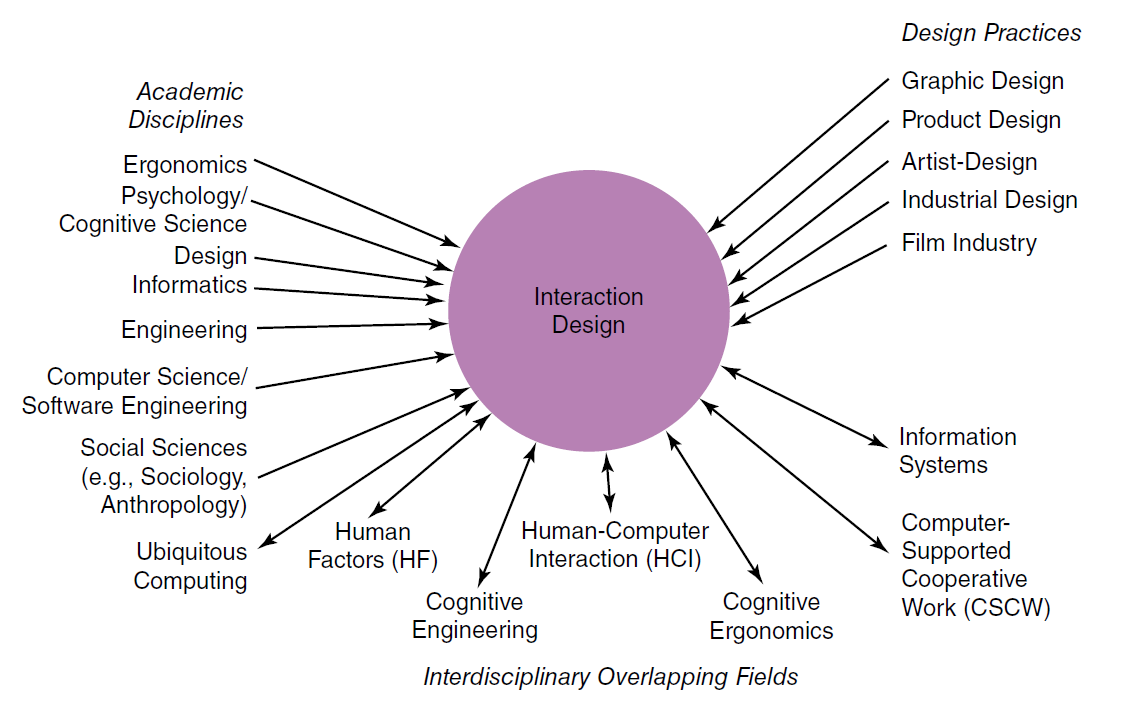
\includegraphics[width=\textwidth]{chapter-2-interaction-design.png}
  \caption{Hubungan studi antardisiplin terkait desain interaksi (Panah dua arah berarti saling tumpang tindih) (Sharp, dkk., 2019)}
  \label{fig:desain_interaksi}
\end{figure}

\subsection{Pendekatan Desain Interaksi}
\label{subsec:pendekatan_id}

Dalam desain interaksi terdapat beberapa pendekatan utama yang dapat digunakan untuk menyusun solusi permasalahan, yaitu \textit{user-centered design} (UCD), \textit{activity-centered design}, \textit{systems design}, dan \textit{genius design}. \parencite{saffer2010designing}

\begin{enumerate}
  \item \textit{User-Centered Design} (UCD)
  \subitem Konsep utama dari UCD adalah mendesain seputar kebutuhan penggunanya. Seorang desainer perlu mendefinisikan tujuan utama dari produk yang dibuat seputar apa yang ingin dicapai oleh penggunanya. Seringkali pengguna pun dilibatkan dalam tahap-tahap pengembangan, seperti pembuatan konsep, pengumpulan data, serta proses pengujian. Hal ini bertujuan untuk menjauhkan produk akhir dari preferensi desainer dan mendekatkan pada preferensi penggunanya sendiri.
   
  \item \textit{Activity-Centered Design}
  \subitem Berbeda dari UCD, pendekatan dengan \textit{activity-centered design} akan memfokuskan seputar kegiatan tertentu. Kegiatan yang dimaksud dapat didefinisikan sebagai kumpulan tugas yang dilakukan untuk mencapai tujuan tertentu. \textit{Activity-centered design} mengharuskan desainer untuk membuat solusi di seputar kegiatan dan menopang kegiatan tersebut, melainkan tujuan dari kegiatan tersebut. Desainer juga harus membedakan maksud dari sebuah aktivitas dengan tujuannya, di mana mereka harus menitikberatkan fokus desain pada maksud dari aktivitas.
 
  \item \textit{Systems Design}
  \subitem \textit{Systems design} adalah pendekatan yang memfokuskan permasalahan pada keseluruhan sebuah sistem dalam proses desainnya. Sistem yang dimaksud bisa terdiri dari banyak komponen pendukung seperti manusia, perangkat keras dan lunak, mesin, dan objek lain sehingga permasalahan yang dihadapi cenderung lebih kompleks.
 
  \item \textit{Genius Design}
  \subitem Pendekatan dengan \textit{Genius Design} mengandalkan sepenuhnya terhadap pengalaman, keahlian, serta preferensi dari desainernya sendiri dalam membuat keputusan desain. Keterlibatan pengguna sangat jarang dan biasanya hanya ada untuk memvalidasi apakah desain yang diprediksi sesuai dengan yang desainer inginkan. Pendekatan ini dinilai memiliki resiko-resiko yang cukup besar namun terkadang dilakukan karena alasan yang lebih kuat daripada resiko tersebut.
 
\end{enumerate}

\subsection{\textit{User-Centered Design} (UCD)}
Seperti yang telah dijelaskan pada subsubbab \ref{subsec:pendekatan_id}, pendekatan UCD memusatkan perhatian proses desain pada pengguna. UCD sendiri merupakan turunan dari cabang ilmu HCI (\textit{Human-Computer Interaction}), yaitu metodologi rekayasa perangkat lunak bagi pengembang yang ditujukan agar perangkat lunak dapat memenuhi kebutuhan penggunanya. \parencite{lowdermilk2013user} Namun pendekatan ini tidak semerta-merta menanyakan langsung keingingan pengguna untuk produknya, karena hal ini dapat membuat produk yang dibuat bias ke pihak tertentu. UCD memiliki tahap dan panduan di mana seorang desainer atau ahli UCD akan mengidentifikasi profil dari penggunanya serta perilaku dan preferensi terhadap aspek-aspek sebuah produk. Informasi yang didapat akan kemudian digunakan dalam proses desain. \parencite{10.1145/1621995.1621997}.

Dalam pendekatan UCD, seorang desainer juga tidak hanya membuat desain dengan tampilan antarmuka yang bagus. Desainer harus memastikan agar desain yang dibuatnya menyelesaikan permasalahan awal sesuai dengan riset yang telah dilakukan dan data yang telah diambil dari pengguna. Desainer bertanggung jawab untuk melakukan evaluasi dengan user untuk memastikan desain yang telah dibuatnya tepat sasaran. \parencite{lowdermilk2013user}

Dalam penerapannya, pendekatan UCD harus mengikuti prinsip-prinsip tertentu. Menurut \textcite{iso9241-210:2010}, berikut adalah prinsip-prinsip standar yang perlu diikuti:

\begin{enumerate}
  \item Desain dibuat berdasarkan pemahaman jelas atas pengguna, tugas-tugas, dan lingkungannya.
  \item Pengguna dilibatkan keseluruhan proses desain dan perkembangannya.
  \item Desain akan diubah dan diperbaiki secara terus-menerus sesuai dengan evaluasi dari pengguna.
  \item Proses UCD dilakukan secara berulang (iteratif).
  \item Desain meliputi keseluruhan \textit{user experience}.
  \item Pembuatan desain melibatkan berbagai perspektif dan kemampuan multidisipliner.
\end{enumerate}

\subsubsection{Proses-Proses dalam UCD}

Dalam melakukan perancangan desain dengan menerapkan pendekatan UCD, terdapat beberapa standar alur pekerjaan yang dapat diikuti. Salah satu yang umum digunakan adalah alur kerja standar ISO 9241-210. Berikut adalah alur kerja UCD sesuai dengan standar ISO 9241-210 yang tercantum pada Gambar II.2.

\begin{figure}[h]
  \centering
  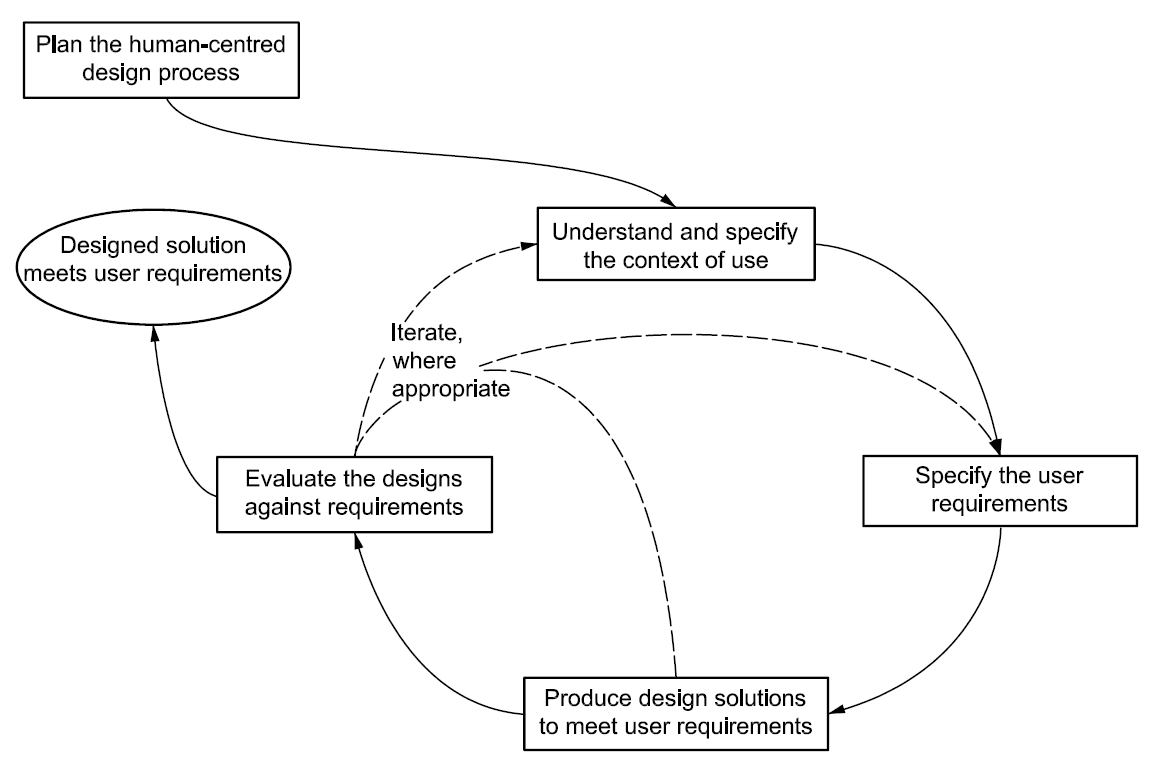
\includegraphics[width=0.9\textwidth]{chapter-2-ucd-figure.png}
  \caption{Alur kerja \textit{User-Centered Design} (ISO 9241-210, 2010)}
  \label{fig:diagram_iso2}
\end{figure}

Terlihat pada diagram alur kerja pada Gambar \ref{fig:diagram_iso2}, terdapat beberapa kegiatan yang dilakukan secara iteratif. Kegiatan-kegiatan yang dilakukan secara iteratif tersebut merupakan komponen utama dalam kerangka UCD. Berikut adalah penjelasan mengenai kegiatan-kegiatan tersebut:

\begin{enumerate}
  \item Memahami dan merincikan konteks penggunaan produk
  \subitem Pada tahap ini dilakukan pengumpulan dan analisa informasi mengenai konteks pemakaian produk. Hal ini bertujuan untuk mengungkapkan adanya kebutuhan, permasalahan, serta batasan dari produk yang penting untuk pengembangan solusi yang akan dibuat. Konteks pemakaian ini perlu mencakup informasi mengenai keseluruhan \textit{stakeholder}, karakteristik target pengguna, tujuan dan kegiatan dari pengguna, serta lingkungan di mana sistem akan dibuat atau dikembangkan.
   
  \item Merincikan kebutuhan pengguna
  \subitem Pada tahap ini dilakukan identifikasi dan analisa lebih lanjut terhadap data-data yang telah dikumpulkan pada tahap sebelumnya. Dari hasil analisa akan didapatkan kebutuhan pengguna yang perlu dipenuhi dalam desain yang akan dibuat nanti. Kebutuhan pengguna yang didapat juga perlu mempertimbangkan batasan yang perlu diikuti sesuai dengan konteks pemakaian produk.
  
  \item Membuat solusi desain yang memenuhi kebutuhan pengguna
  \subitem Tahap selanjutnya adalah membuat prototipe desain sesuai dengan kebutuhan pengguna yang telah diidentifikasi pada fase sebelumnya. Prototipe desain yang dimaksud adalah produk implementasi desain aplikasi yang sudah menyerupai produk akhir, tanpa adanya implementasi unsur-unsur teknikal aplikasi tersebut. Hal ini bertujuan agar pengguna dapat memahami interaksi dan antarmuka dari desain aplikasi untuk dievaluasi pada tahap selanjutnya sebelum menjalani implementasi akhir.
  
  \item Mengevaluasi desain yang dibuat terhadap kebutuhan
  \subitem Proses evaluasi adalah proses untuk menentukan apakah desain aplikasi yang dibuat telah menyelesaikan permasalahan atau memenuhi kebutuhan yang diidentifikasi pada tahap-tahap sebelumnya. Proses evaluasi juga dilakukan untuk mengetahui apakah desain aplikasi sesuai dengan \textit{user experience goals} dan \textit{usability goals} yang diharapkan. Proses evaluasi tidak menutup kemungkinan adanya wawasan baru mengenai kebutuhan pengguna atau desain aplikasinya sendiri. Hasil dari evaluasi akan menentukan apakah desain tersebut layak dilanjutkan ke tahap implementasi atau diperlukan iterasi untuk menjalani perbaikan.

\end{enumerate}



\section{\textit{Usability Goals} dan \textit{User Experience Goals}}
Untuk mendesain produk yang tepat bagi pengguna, seorang desainer perlu mengerti kebutuhan pengguna dengan menentukan tujuan yang jelas dari pengembangan produk interaktif tersebut. \textcite{sharp2019interaction} menyebutkan bahwa untuk mencapainya, tujuan dapat diklasifikasikan sesuai dengan \textit{usability goals} dan \textit{user experience goals}.

% http://bpm.umg.ac.id/aset/images/download/M4-Standar-Rujuka-BA(1-8-2017).pdf


\textit{Usability goals} mengarahkan produk untuk mencapai kriteria \textit{usability} tertentu. \textit{Usability goals} mencakup bagaimana cara untuk mengoptimalisasi interaksi pengguna dengan produk untuk melakukan kegiatannya. \textit{Usability goals} dapat diuraikan menjadi 6 tujuan berikut:
\begin{enumerate}
  \item Efektif untuk digunakan (\textit{effectiveness}) adalah tujuan yang menunjukkan apakah suatu produk sukses dalam menjalankan tugasnya.
  \item Efisien untuk digunakan (\textit{efficiency}) adalah tujuan yang menunjukkan bagaimana sebuah produk dapat membantu pengguna dalam mencapai tujuannya. Sebuah produk dapat dikatakan efisien jika penggunanya dapat melakukan suatu kegiatan dalam langkah-langkah yang sederhana dan tidak menuntut pengguna untuk mempelajari langkah-langkah tersebut terlalu lama.
  \item Aman untuk digunakan (\textit{safety}) adalah tujuan yang menunjukkan bagaimana sebuah produk dapat melindungi penggunanya dari situasi yang berbahaya atau tidak diinginkan, atau melakukan hal-hal yang bersifat destruktif. Tujuan ini dapat dicapai dengan meminimalisir resiko yang dapat ditemui pengguna atau memberikan opsi untuk membatalkan aksinya. Tujuan ini juga menunjukkan bagaimana sebuah produk membantu penggunanya mengeksplorasi produk secara percaya diri.
  \item Memiliki utilitas yang baik (\textit{utility}) adalah tujuan yang menunjukkan bagaimana sebuah produk menyediakan fungsionalitas yang baik untuk membantu pengguna melakukan hal yang dibutuhkan atau diinginkan.
  \item Mudah untuk dipelajari (\textit{learnability}) adalah tujuan yang menunjukkan seberapa mudah sebuah produk untuk dipelajari hingga pengguna dapat menggunakannya dengan benar.
  \item Mudah untuk mengingat penggunaan (\textit{memorability}) adalah tujuan yang menunjukkan seberapa mudah bagi pengguna untuk mengingat bagaimana cara menggunakan sebuah produk setelah mempelajarinya.
\end{enumerate}


\textit{User experience goals} lebih bersifat subjektif dibandingkan \textit{usability goals} karena mencakup berbagai jenis emosi dan pengalaman yang dirasakan oleh pengguna saat berinteraksi dengan produk. \textit{User experience goals} juga berhubungan erat dengan estetika dari produk. \textit{User experience goals} terdiri dari 2 jenis, yaitu tujuan yang diharapkan dan tujuan yang tidak diharapkan. \parencite{sharp2019interaction} Pembagiannya dapat dilihat pada Tabel \ref{tab:ux_goals}.

\begin{table}[h]
  \fontsize{10}{12}
  \caption{\textit{User experience goals} yang diharapkan dan tidak diharapkan}
  \label{tab:ux_goals}
  \vspace{0.25cm}
  \begin{center}
      \begin{tabular}{|l|l|}
            \hline
            \textit{User experience goals} yang diharapkan & \textit{User experience goals} yang tidak diharapkan \tabularnewline
            \hline
            1.	Satisfying              & 1.  Boring                  \tabularnewline
            2.	Helpful                 & 2.  Unpleasant              \tabularnewline
            3.	Fun                     & 3.  Frustrating             \tabularnewline
            4.	Enjoyable               & 4.  Patronizing             \tabularnewline
            5.	Motivating              & 5.  Making one feel guilty  \tabularnewline
            6.	Provocative             & 6.  Making one feel stupid  \tabularnewline
            7.	Engaging                & 7.  Annoying                \tabularnewline
            8.	Challenging             & 8.  Cutesy                  \tabularnewline
            9.	Surprising              & 9.  Childish                \tabularnewline
            10.	Pleasurable             & 10. Gimmicky                \tabularnewline
            11.	Enhancing sociability   &                             \tabularnewline
            12.	Rewarding               &                             \tabularnewline
            13.	Exciting                &                             \tabularnewline
            14.	Supporting creativity   &                             \tabularnewline
            15.	Emotionally fulfilling  &                             \tabularnewline
            16.	Entertaining            &                             \tabularnewline
            17.	Cognitively stimulating &                             \tabularnewline
            18.	Experiencing flow       &                             \tabularnewline
            \hline
        \end{tabular}
    \end{center}
\end{table}


% \section{Usability Testing}
% Usability Testing adalah sebuah proses pengujian produk yang sedang dikembangkan untuk mengetahui apakah produk tersebut dapat digunakan dengan benar oleh pengguna yang terpilih, serta untuk menguji kepuasan pengguna dalam menggunakan produk. Dengan melakukan usability testing di sebuah lingkungan yang terkendali, desainer atau peneliti dapat mengendalikan pengaruh lingkungan yang dapat mempengaruhi performa pengguna. \parencite{sharp2019interaction}

% Menurut \textcite{moran2019usabilitytest}, \textit{usability testing}, yang seringkali disebut juga \textit{user testing}, adalah suatu metodologi riset yang digunakan untuk mengidentifikasi masalah dalam sebuah desain produk atau layanan, menemukan celah atau ruang untuk perbaikan, serta mempelajari perilaku dan preferensi dari pengguna target produk. Dalam proses \textit{usability testing}, terdapat 3 elemen utama:
% \begin{enumerate}
%   \item Fasilitator
%   \subitem
%   Seorang fasilitator akan membimbing partisipan melalui proses pengujian, di mana dia akan memberikan instruksi-instruksi, menjawab pertanyaan partisipan, dan memberikan pertanyaan kepada partisipan. Fasilitator bertugas untuk memastikan bahwa data yang didapat dari pengujian memilki kualitas yang tinggi dan bersifat sah, tanpa mempengaruhi sikap dan tindakan pengguna saat mengerjakan pengujian.
  
%   \item Tugas
%   \subitem
%   Dalam melakukan pengujian, partisipan akan diberikan tugas-tugas realistis yang dapat dilakukan pada produk akhir di dunia nyata. Susunan kata pada tugas ini sangat penting, kesalahan penulisan atau pengguna frase dapat memberikan pengertian yang salah kepada pengguna dan dapat mempengaruhi sikap pengguna dalam menguji produk. 

%   \item	Partisipan
%   \subitem
%   Partisipan dari pengujian ini bermaksud sebagai pengguna realisitis yang masuk ke dalam target pemasaran produk, hal ini dapat berarti para partisipan memiliki latar belakang yang sama atau kebutuhan yang sama. Partisipan kemungkinan pernah memakai produknya, atau belum pernah sama sekali. Selama mengerjakan tugas, partisipan seringkali diperintahkan untuk mengatakan apa langkah yang sedang dilakukan untuk membantu penguji dalam mencatat data dan memastikan bahwa partisipan melakukan tugasnya sesuai dengan maksud penguji.
% \end{enumerate}

% \subsection{Sifat Usability Testing}
% Moran melanjutkan bahwa \textit{usability testing} memiliki sifat-sifat yang terbagi berdasarkan 2 kategori, yaitu:

% \begin{enumerate}
%   \item Data yang dikumpulkan
%   \subitem \textit{Usability testing} dapat dibagi berdasarkan data seperti apa yang ingin dikumpulkan. \textit{Qualitative usability testing} adalah pengujian yang berfokus untuk mengumpulkan wawasan dan temuan pengguna saat memakai produk. Pengujian ini cocok untuk menemukan masalah-masalah dalam pengalaman pengguna. \textit{Quantitative usability testing} adalah pengujian yang berfokus untuk mengumpulkan metrik yang digunakan untuk menjelaskan pengalaman pengguna. Metrik yang paling umum dikumpulkan adalah keberhasilan dan waktu pengerjaan tugas. Pengujian ini cocok untuk mengumpulkan tolok ukur.
  
%   \item Lokasi \textit{usability testing}
%   \subitem 
%   \textit{Usability testing} dapat dibagi berdasarkan lokasi pengguna dan pengamat saat melakukan pengujian. \textit{In-person usability testing} adalah pengujian di mana pengguna dan penguji berada di lokasi yang sama. Mereka tidak perlu berada di ruangan yang sama, namun pengamat dapat mengobservasi pengguna secara langsung. \textit{Remote usability testing} adalah pengujian di mana pengguna dan pengamat berada di lokasi yang berbeda. Pengujian ini lebih sering dipakai karena biayanya yang murah dan waktu yang diperlukan lebih singkat. Pengujian ini dapat dibagi lagi berdasarkan moderasi yang dilakukan selama pengujian berlangsung. Pada \textit{remote moderated usability testing} pengamat tetap mengobservasi pengguna namun melalui aplikasi konferensi online, sedangkan pada \textit{remote unmoderated usability testing} pengguna menggunakan kakas \textit{remote-testing} untuk mengerjakan tugas-tugas yang teWlah diberikan dan menanyakan pertanyaan lanjutan, kemudian rekaman sesi pengerjaan dan metrik yang didapat akan dikirim kepada penguji.
% \end{enumerate}

% \section{Keamanan Informasi}
% \textcite{andress2014basics} mengutip dari pemerintah Amerika Serikat, keamanan informasi adalah tindakan perlindungan informasi dan sistem informasi dari pengaksesan, penggunaan, penyingkapan, perubahan, dan pengrusakan yang tidak diizinkan. Andress meneruskan bahwa perlindungan yang dimaksud dapat terhadap serangan terhadap jaringan, bencana alam, kondisi lingkungan, kegagalan listrik, pencurian atau vandalisme, atau kondisi lainnya. Dalam sebuah usaha untuk melindungi informasi, dapat dipertimbangkan aset apa saja yang penting untuk diamankan, baik dari segi fisik maupun segi yang lebih rentan seperti perangkat lunak, kode, atau data.

% \subsection{Model Fundamental Keamanan Informasi}
% Terdapat model yang digunakan sebagai fundamental dalam merancang konsep keamanan informasi yang disebut sebagai CIA Triad. Kegagalan terhadap salah satu komponen dalam model CIA Triad dapat berarti kegagalan dalam keamanan informasi. Model CIA Triad terdiri dari Confidentiality, Integrity, dan Availability. \parencite{andress2014basics}
% \begin{figure}[h]
%   \centering
%   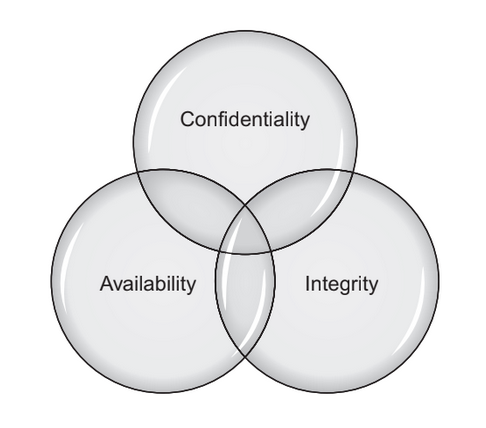
\includegraphics[width=0.5\textwidth]{chapter-2-model-CIA-triad.png}
%   \caption{Model CIA Triad}
% \end{figure}

% \begin{enumerate}[label=\alph*.]
%   \item \textit{Confidentiality}
%   \subitem 
%   \textit{Confidentiality} atau kerahasiaan adalah komponen penting dalam privasi yang berarti kemampuan sistem dalam melindungi data dari pihak yang tidak diizinkan. \textit{Confidentiality} dapat gagal ketika suatu pihak mendapatkan akses terhadap data yang dilindungi, misalnya dengan seseorang mengintip layar yang tertera data tersebut, atau data yang tidak sengaja dikirim lewat email kepada orang yang salah. 

%   \item \textit{Integrity}
%   \subitem
%   \textit{Integrity} atau integritas adalah kemampuan dalam mencegah data dari perubahan yang tidak diizinkan. Perubahan data yang dimaksud dapat berupa diubahnya atau dihapusnya sebagian atau seluruh data yang tidak diizinkan. \textit{Integrity} juga dapat gagal bila terjadi data diizinkan untuk diubah atau dihapus, namun tidak diinginkan. Hal ini berarti diperlukan sebuah mekanisme untuk membatalkan perubahan yang telah dilakukan selain mencegah dari perubahan yang tidak diinginkan.

%   \item \textit{Availability}
%   \subitem
%   \textit{Availability} atau ketersediaan adalah kemampuan untuk mengakses data ketika dibutuhkan. Kehilangan akses terhadap 1 buah data dapat merusak rantai pada sebuah sistem yang memerlukan akses terhadap data tersebut. Kegagalan terhadap \textit{availability} dapat terjadi karena kegagalan listrik, kegagalan sistem operasi, serangan jaringan, sistem yang tersusupi, atau masalah lain.

% \end{enumerate}

% \section{OWASP Top10}
% OWASP atau Open Web Application adalah sebuah komunitas terbuka yang berfokus pada keamanan di internet. OWASP mendedikasikan diri untuk memungkinkan organisasi-organisasi untuk mengembangkan, membeli, dan memelihara aplikasi dan API yang dapat dipercaya. Selain itu, OWASP membuat sebuah daftar 10 resiko kritis teratas yang dapat mengancam keamanan aplikasi web di internet, daftar ini disebut dengan OWASP Top10. Sejak tahun 2021, daftar ini terdiri atas:
% \begin{enumerate}
%   \item A01:2021 – Broken Access Control
%   \item A02-2021 – Cryptographic Failures
%   \item A03-2021 – Injection
%   \item A04-2021 – Insecure Design
%   \item A05-2021 – Security Misconfiguration
%   \item A06-2021 – Vulnerable and Outdated Components
%   \item A07-2021 – Identification and Authentification Failures
%   \item A08-2021 – Software and Data Integrity Failures
%   \item A09-2021 – Security Logging and Monitoring Failures
%   \item A10-2021 – Server-side Request Forgery (SSRF)
% \end{enumerate}

% \section{Privasi Informasi}
% Menurut Dr. Alan F. Westin yang dikutip oleh \textcite{givens2014information}, privasi sebuah klaim oleh individual, grup, atau institusi untuk menentukan sendiri kapan, bagaimana, dan sejauh apa informasi tentang mereka dapat dikomunikasikan kepada pihak lain. Givens meneruskan bahwa privasi informasi adalah subset dari pengertian privasi yang disebutkan oleh Westin. Givens mengutip Peter P. Swire dan Kenesa Ahmad bahwa ada 4 kelas dari privasi, yiatu privasi komunikasi, privasi wilayah, privasi tubuh, dan privasi informasi yang berarti perhatian terhadap pendirian ketentuan-ketentuan yang mengatur pengumpulan dan penanganan dari informasi pribadi, termasuk informasi medis dan finansial.
